\chapter{\label{Intro}Introduction}

The rendering problem of calculating the radiance  (brightness) of all surfaces in 3D scene is very important in 3D computer graphics. Given a geometrical location and optical characteristics  (reflectivity) of surfaces along with light sources (emitters) in 3D scene our concern is to calculate radiance and generate realistic image of scene illuminated with light source.

\section{Direct and Indirect illumination}
There are two types of renderer, direct illumination renderer and indirect illumination renderer. 
Figure \ref{fig:directindirect} shows an example of difference between direct and indirect illumination. The image on the left in the figure is rendered with standard direct illumination renderer. It consist of mainly two lighting effects, first one is light received directly from light source and second one is ambient light without which surfaces which are not directly illuminated will be completely dark.\underline{ decide whether two lighting efect or 3 as in wikipedia}. Image on the right of Figure \ref{fig:directIndirect} is rendered by indirect illumination renderer. Clearly, image generate using indirect illumination renderer generates more realistic images.
\begin{figure}[tbh]
\centering{}
\captionsetup{justification=centering}
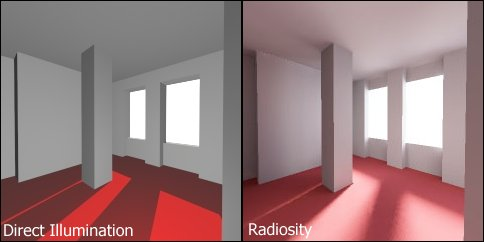
\includegraphics[width=5in]{DirectIndirect.jpg}
\caption{\label{fig:directindirect}Difference between direct illumination and indirect illumination \cite{wikiradiosity}}
\end{figure}

Global illumination or indirect illumination is a name for a group of algorithms  (renderer) used in 3D computer graphics that are meant to add more realistic lighting to 3D scenes. Such algorithms take into account not only the light energy which comes directly from a light source  (direct illumination), but also light energy from the same source which are reflected by other surfaces in the scene  (indirect illumination). As a result global illumination adds realistic features like light bouncing  (multiple inter-reflection between two surfaces) and color bleeding, between pair of adjacent surfaces. A well known global illumination algorithm is ray-tracing \cite{Whitted}, which computes  radiance of the area of the surface of the scene seen from one given viewpoint. In other words, it only calculates radiance of points which are visible in final image. Thus for changing the viewpoint of scene we need to run algorithm again, making it viewpoint dependent.

\section{Radiosity}

Radiosity algorithms are set of global illumination algorithms calculating radiance of surfaces reflecting light diffusely (equal apparent brightness in all the directions above the surface). In other words, radiosity takes the 3D scenes with Lambertian surfaces as input. Lambertian reflectance is the property of an ideal "matte" or diffusely reflecting surface. Opposite to ray-tracing, radiosity calculates radiance of all points in the scene. This allows the computation to be viewpoint independent i.e. solution for given scene can be used to generate images of scene from arbitrary viewpoint. This is advantage as well as drawback as we need to do extra work to find radiance of all the points. Radiosity also refers to measure of power per unit area at a point. Thus solution of the this problem is radiosity function over the domain of surfaces in the scene. 




\section{Organization of the Report}
{\bf Describe the sections}